\documentclass[review]{elsarticle}

\usepackage{lineno}
\usepackage{xspace}
\modulolinenumbers[5]

\journal{Annals of Nuclear Energy}

%% `Elsevier LaTeX' style
\bibliographystyle{elsarticle-num}
%%%%%%%%%%%%%%%%%%%%%%%

%%%% packages and definitions (optional)
\usepackage{placeins}
\usepackage{booktabs} % nice rules (thick lines) for tables
\usepackage{microtype} % improves typography for PDF
\usepackage{hhline}
\usepackage{amsmath}

%\usepackage[demo]{graphicx}
%\usepackage{caption}
%\usepackage{subcaption}

\usepackage{booktabs}
\usepackage{threeparttable, tablefootnote}

\usepackage{tabularx}
\newcolumntype{b}{>{\hsize=1.0\hsize}X}
\newcolumntype{s}{>{\hsize=.5\hsize}X}
\newcolumntype{m}{>{\hsize=.75\hsize}X}
\newcolumntype{x}{>{\hsize=.25\hsize}X}

%\newcommand{\Cyclus}{\textsc{Cyclus}\xspace}%
%\newcommand{\Cycamore}{\textsc{Cycamore}\xspace}%
\graphicspath{ {../figures/} }

% tikz %
\usepackage{tikz}
\usetikzlibrary{positioning, arrows, decorations, shapes}

\usetikzlibrary{shapes.geometric,arrows}
\tikzstyle{process} = [rectangle, rounded corners, minimum width=3cm, minimum height=1cm,text centered, draw=black, fill=blue!30]
\tikzstyle{object} = [ellipse, rounded corners, minimum width=3cm, minimum height=1cm,text centered, draw=black, fill=green!30]
\tikzstyle{arrow} = [thick,->,>=stealth]

% hyperref %
\usepackage[hidelinks]{hyperref}

\begin{document}
\begin{frontmatter}
\title{Graphical Abstract\\
Modeling and Simulation of Online Reprocessing in the Thorium-Fueled Molten Salt Breeder Reactor}
\date{}                     %% if you don't need date to appear

\end{frontmatter}

\begin{figure}[htbp!]
    \begin{center}
        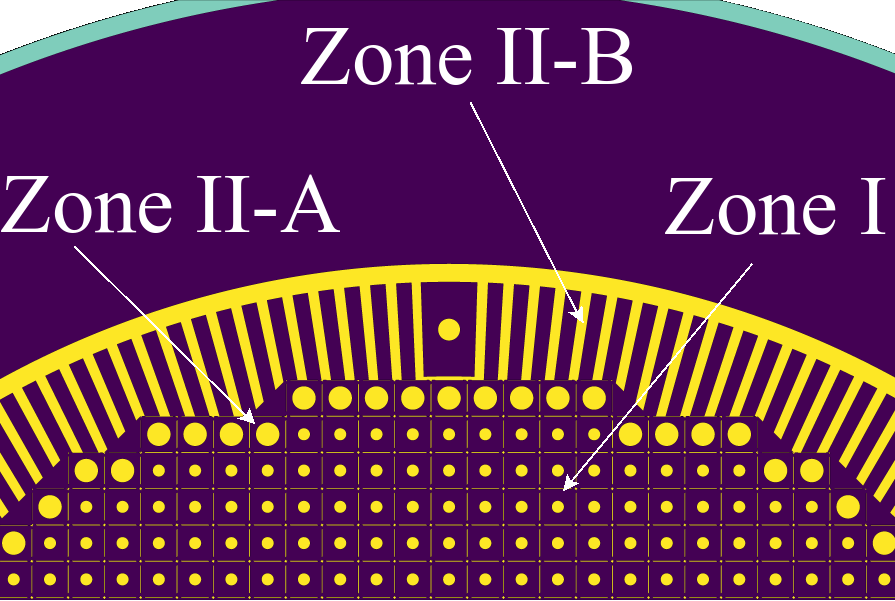
\includegraphics[width=0.49\textwidth]{ser_zone_II.png}
        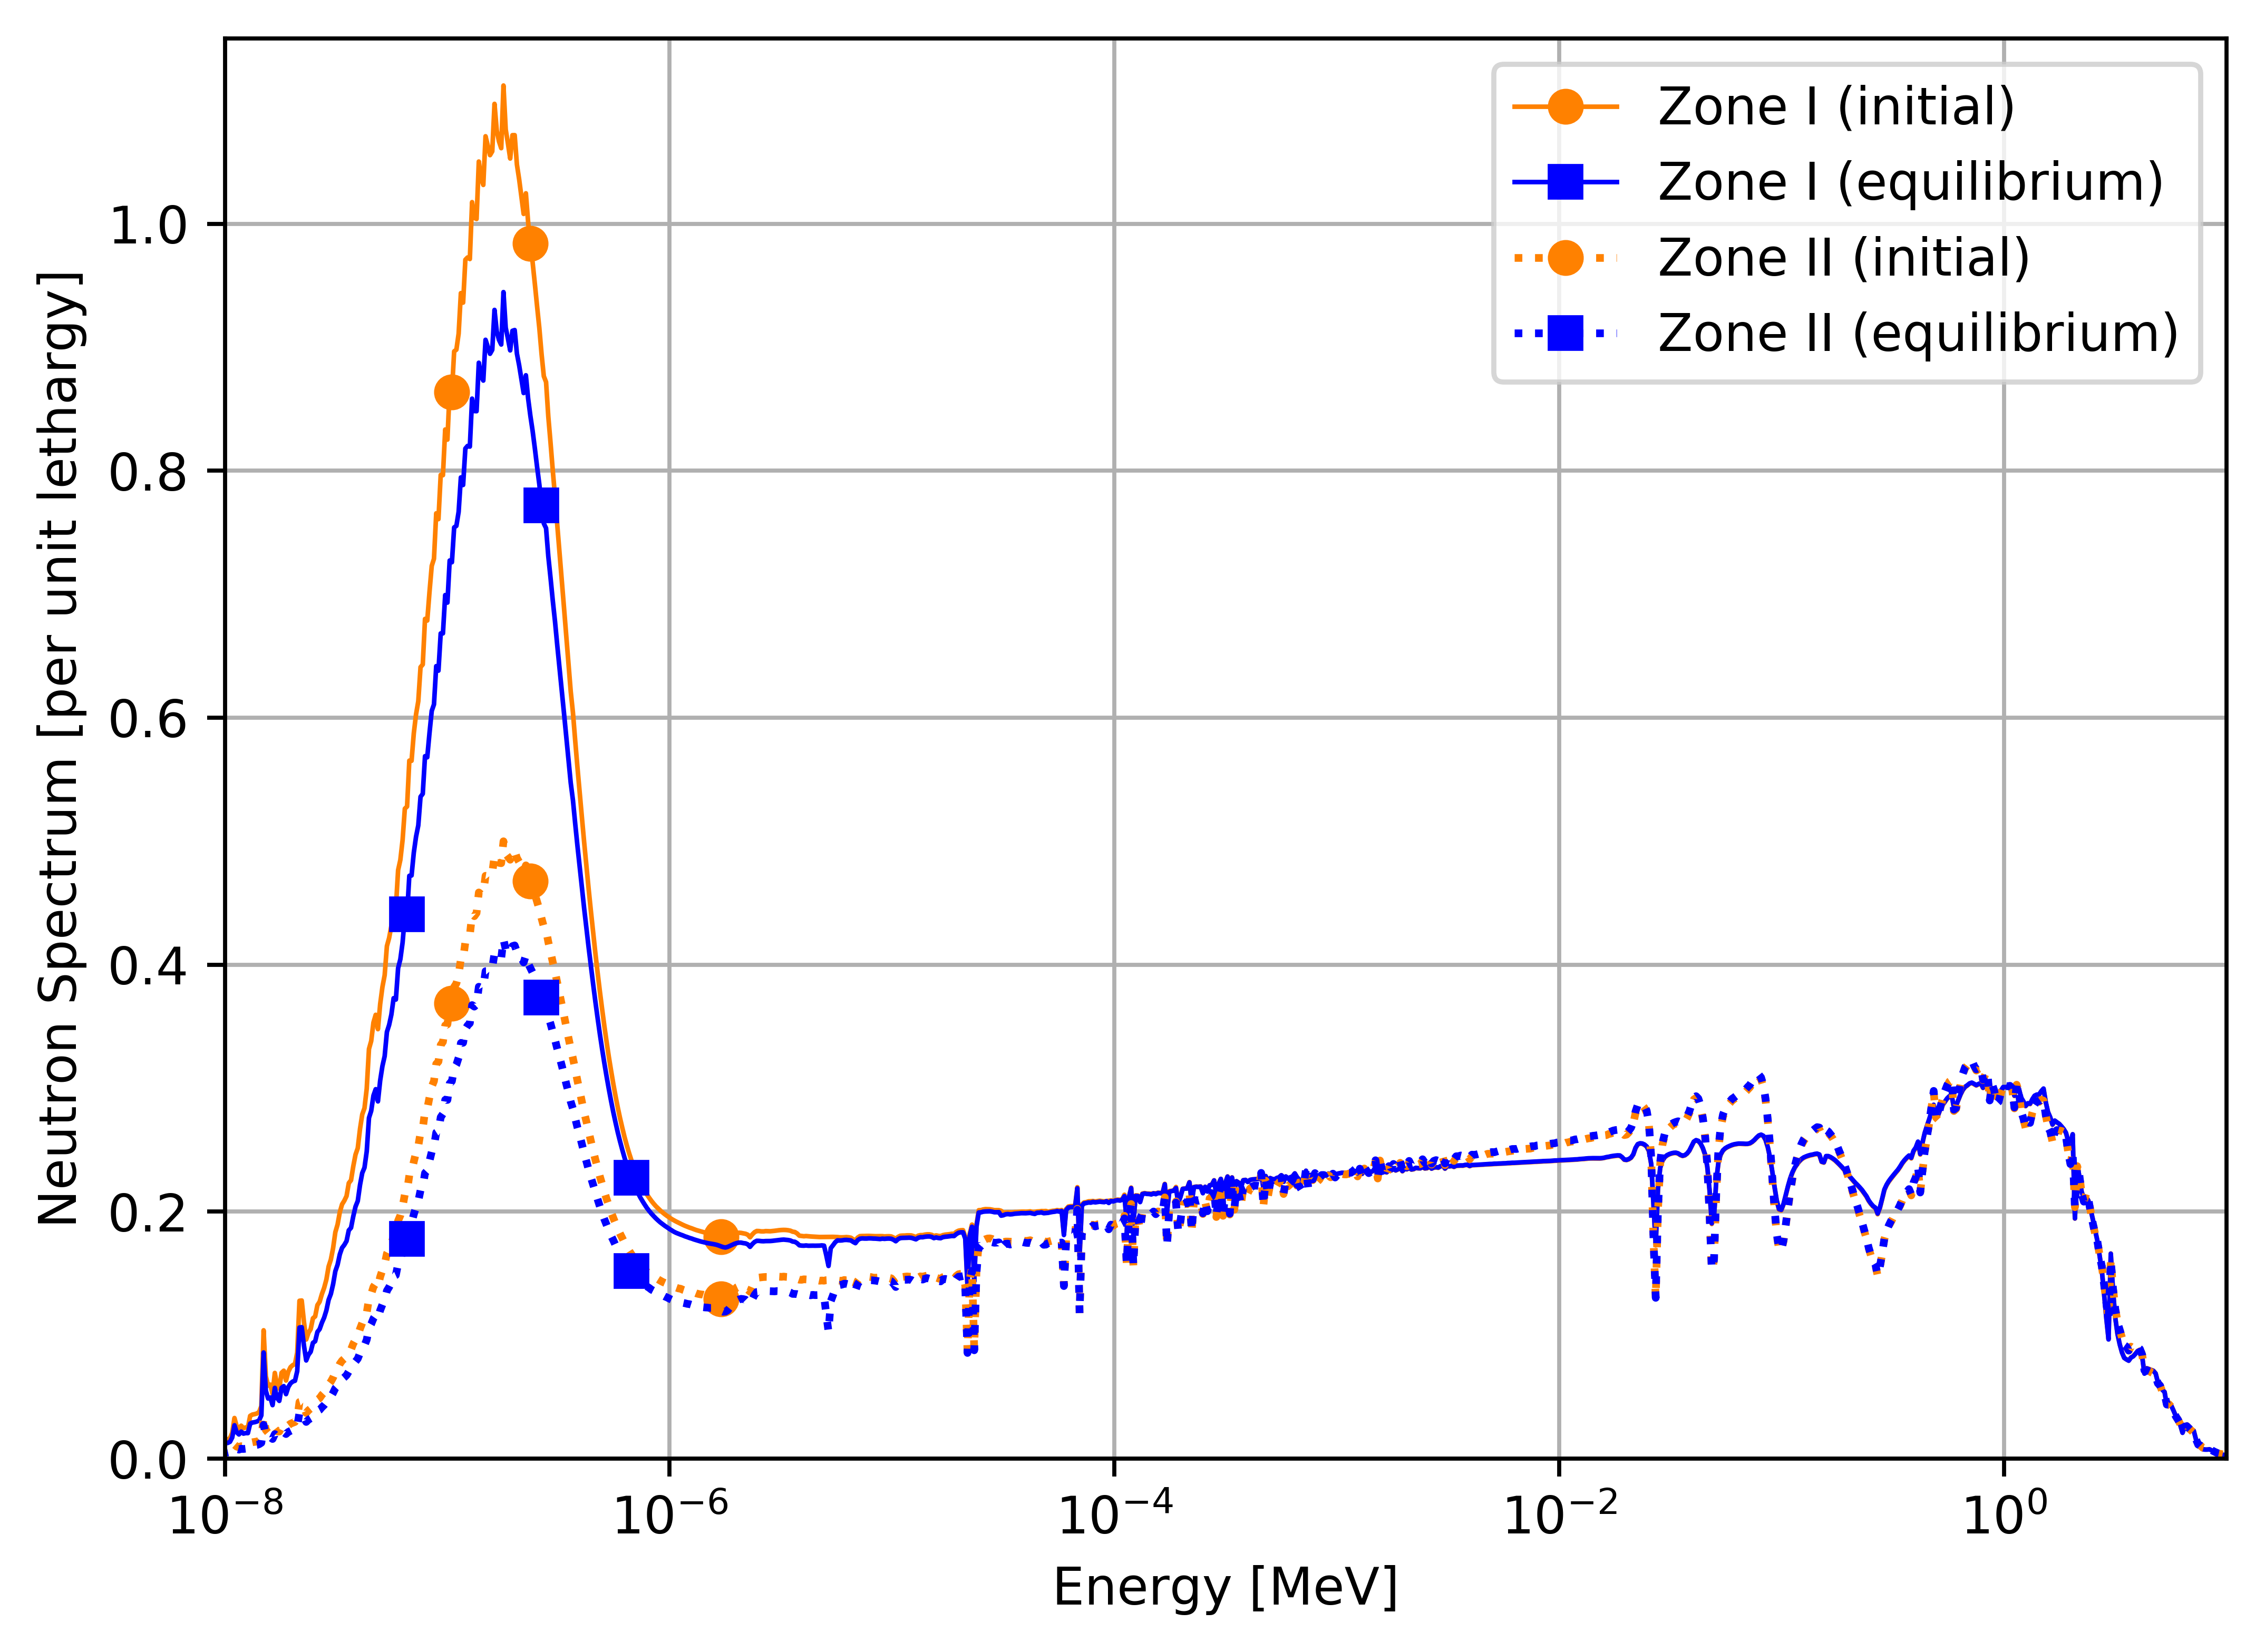
\includegraphics[width=0.49\textwidth]{spectrum_zones.png}
    \end{center}
    \label{fig:graph-abs}
    \caption{The Molten Salt Breeder Reactor (left) was modeled in full
three-dimensional detail.  Yellow represents fuel salt, purple represents
graphite, and aqua represents the reactor vessel Online liquid fuel processing
was simulated until a quasi-equillibrium of fuel composiion could be
established. Reactor physics parameters, such as flux profiles, were evaluated
during the 10 year evolution.}
\end{figure}

\end{document}
